\section{Examples of methods}\label{sec:examples-methods}
In this section we will present how the linear and nonlinear methods behave on linear and nonlinear data. It should be noted again that the methods have different purposes. As a quick reminder \gls{pca} tries to maximize the variance in the embedded data (and so does \gls{kpca}), while \gls{lda} tries to maximize the separability of classes in the data, and \gls{isomap} tries to preserve the distances from the high-dimensional data when projecting it onto a lower space. Therefore their results will not a one-to-one comparison.


\subsection{Linear data example}\label{subsec:linear-data-example}
As linear data we will use the Iris dataset, which contains three different species of Iris flowers, with 50 examples each. Each class has four dimensions, which are the length and width of the sepals, and petals ~\cite{iris-dataset}. The dataset is a simple and well-known dataset, which has been used in many machine learning papers ~\cite{iris-dataset}, and should give intuition as to how the methods behave on the dataset.

\begin{figure}[htb!]
\centering
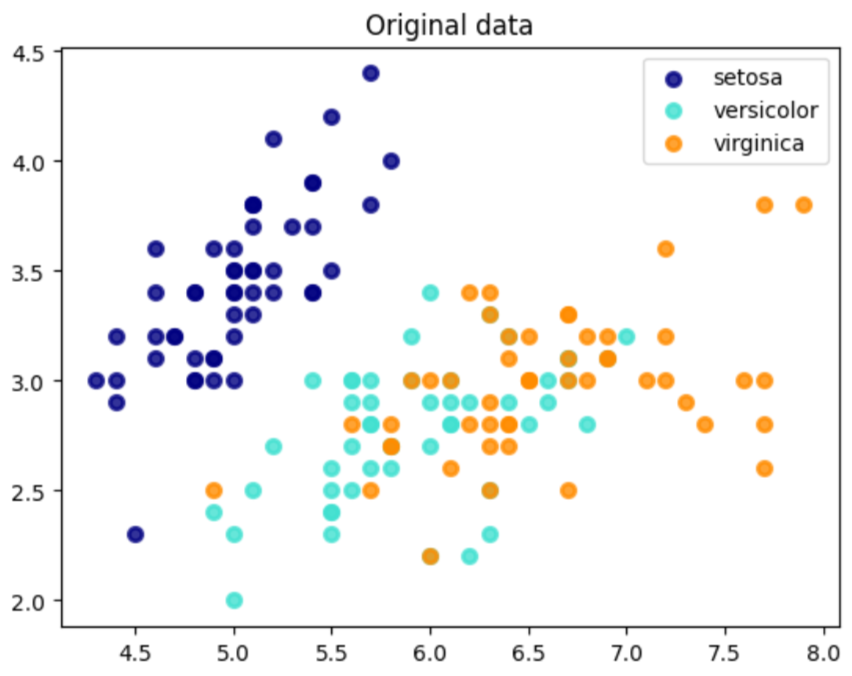
\includegraphics[width=0.5\textwidth]{figures/theory-example-figures/linear-data.png}
\caption{Linear data as Iris dataset}
\label{fig:linear-data}
\end{figure}

On figure \ref{fig:linear-data} the iris flowers are represented on a 2D plot. According to ~\cite{iris-dataset} only one class is separable, and that can further be  solidified by the fact that the species setosa is the only class that is visually linearly separable.

\subsubsection{Linear methods}\label{subsubsec:linear-methods-on-iris}
On figure \ref{fig:iris-pca} one can see that \gls{pca} has successfully separated the setosa species from the other classes in the dataset. With respect to the other species, on the coordiantes [1.20, 0.20] they do not seem to be clearly separated.

\begin{figure}[htb!]
\centering
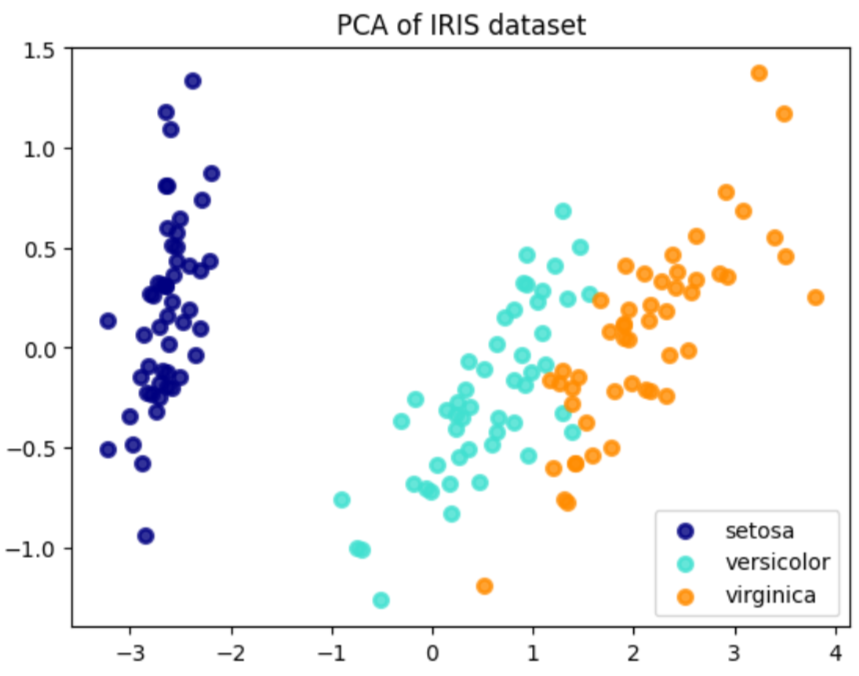
\includegraphics[width=0.5\textwidth]{figures/theory-example-figures/iris-pca.png}
\caption{PCA on iris}
\label{fig:iris-pca}
\end{figure}


\begin{figure}[htb!]
    \centering
    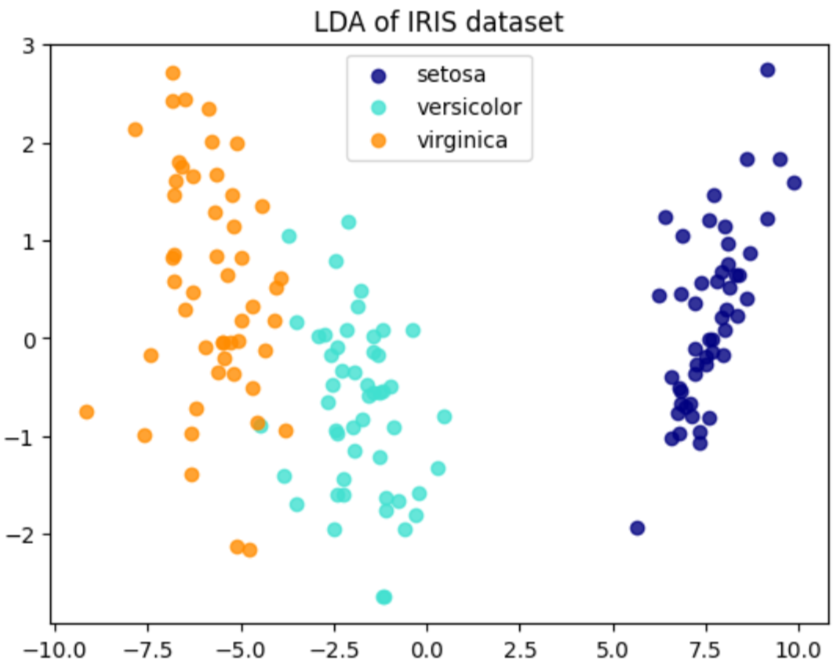
\includegraphics[width=0.5\textwidth]{figures/theory-example-figures/iris-lda.png}
    \caption{LDA on iris}
    \label{fig:iris-lda}
    \end{figure}
    
On figure \ref{fig:iris-lda} \gls{lda} has also successfully separated the setosa species from the other classes in the dataset. In contrast with \gls{pca}, \gls{lda} has managed to separate somewhat better as the distinction between those classes can be made easier. An advantage, which \gls{lda} poses, is that \gls{lda} is a supervised method, which means that LDA knows the labels of the data, and therefore may be better suited for classifying the data.

\subsubsection{Nonlinear methods}\label{subsubsec:nonlinear-methods-on-iris}
On figure \ref{fig:iris-isomap} \gls{isomap} has tried to separate the setosa, and managed to map the data on the first two dimensions. \gls{isomap}, as opposed to the aforementioned linear methods, has not found too much diversity on the second projection, as the values range from approximative 0.0 to -0.25. Such range is short in comparison with the linear methods. Isomap clusters the setosa species, but that may not be helpful if the data needs to be projected on two dimensions. If, for example, a point is in upper left corner, then it is not possible to tell if it is a setosa, or a versicolor. \gls{isomap} is nevertheless a nonlinear method, and it is expected that it does not reduce the data as efficiently as the linear methods do.

\begin{figure}[htb!]
    \centering
    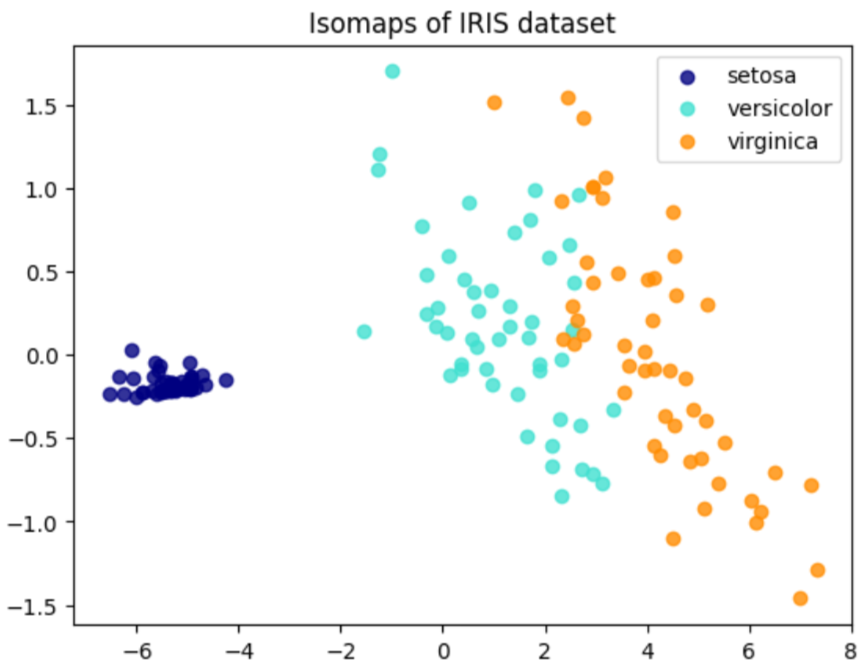
\includegraphics[width=0.5\textwidth]{figures/theory-example-figures/iris-isomap.png}
    \caption{Isomap on iris}
    \label{fig:iris-isomap}
    \end{figure}

On figure \ref{fig:iris-kernelpca} \gls{kpca} has tried to separate the setosa. On the figure it can be seen that \gls{kpca} has clustered the other two species on the first projection, but there cannot be seen any clear separation between the two species, especially on the second projection. \gls{kpca} has also mapped the data points for setosa with a high degree of variance, but it did not clearly separate the setosa from the other two species. Likewise \gls{isomap}, \gls{kpca} was not supposed to separate the data as good as the linear methods, but it is interesting that KernelPCA has not managed to fully separate the setosa species from the rest of the data.

\begin{figure}[htb!]
    \centering
    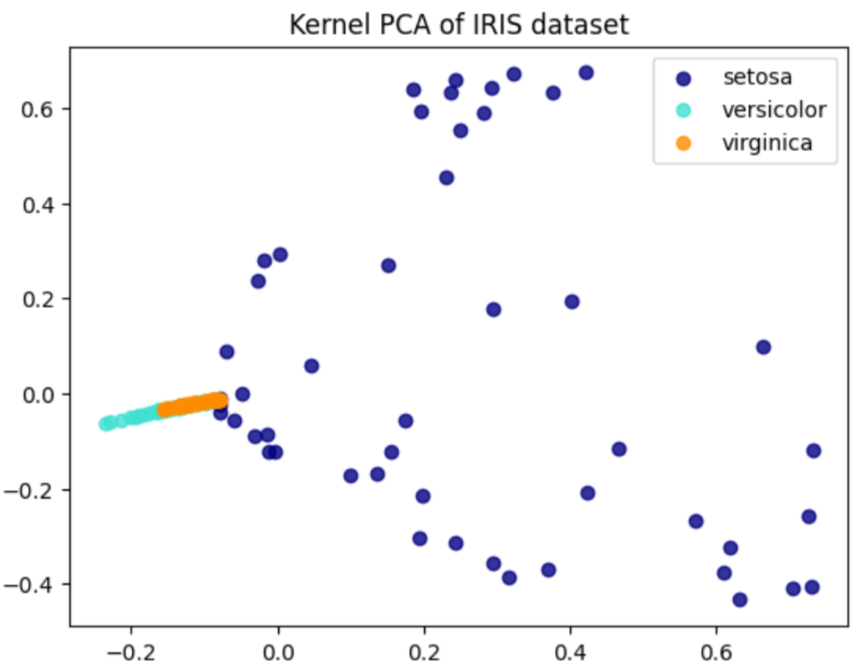
\includegraphics[width=0.5\textwidth]{figures/theory-example-figures/iris-kernelpca.png}
    \caption{KernelPCA on iris}
    \label{fig:iris-kernelpca}
    \end{figure}

\subsection{Nonlinear data example}\label{subsec:nonlinear-data-example}
As nonlinear data we will construct two different classes of cirlces, an inner- and outer circle, which will look like in the figure ~\ref{fig:circles}.

\begin{figure}[htb!]
    \centering
    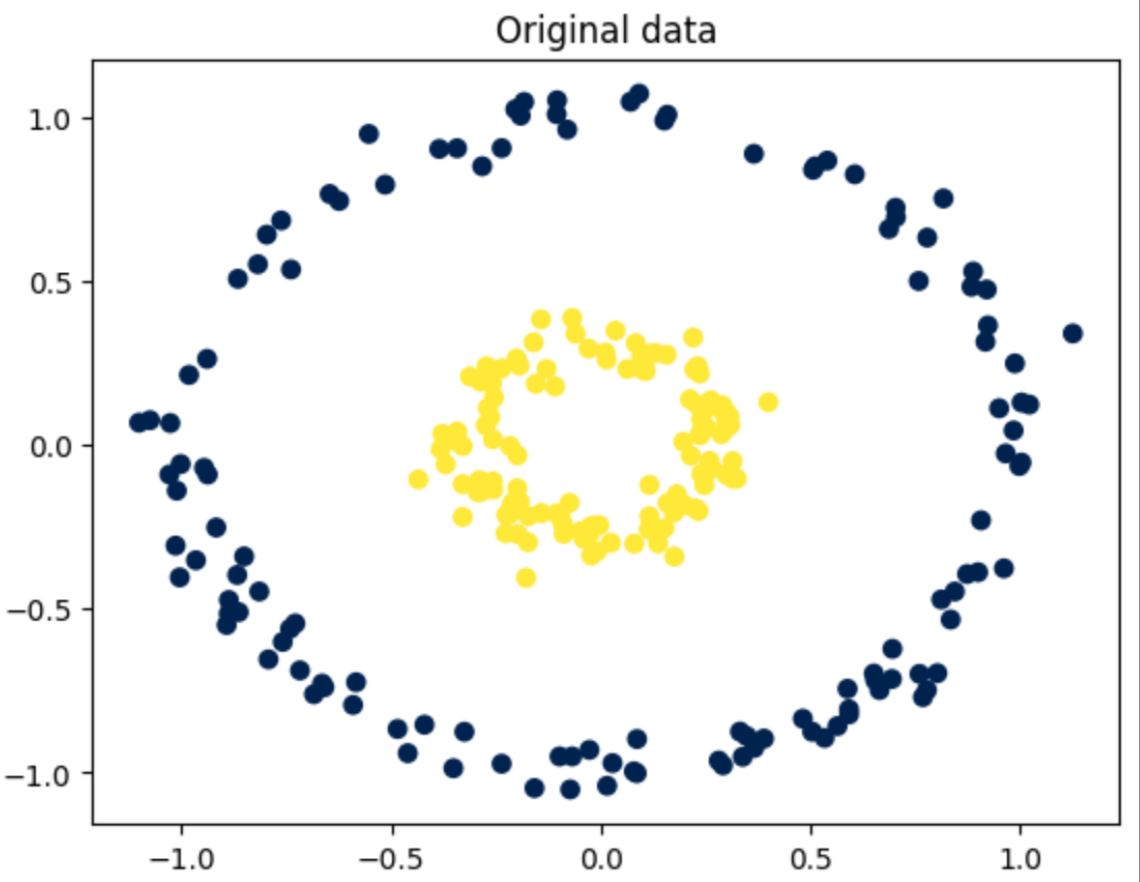
\includegraphics[width=0.5\textwidth]{figures/theory-example-figures/fig-circles.png}
    \caption{Nonlinear data as two circles}
    \label{fig:circles}
    \end{figure}

\subsubsection{Linear methods}\label{subsubsec:linear-methods-on-circles}
\begin{figure}[htb!]
    \centering
    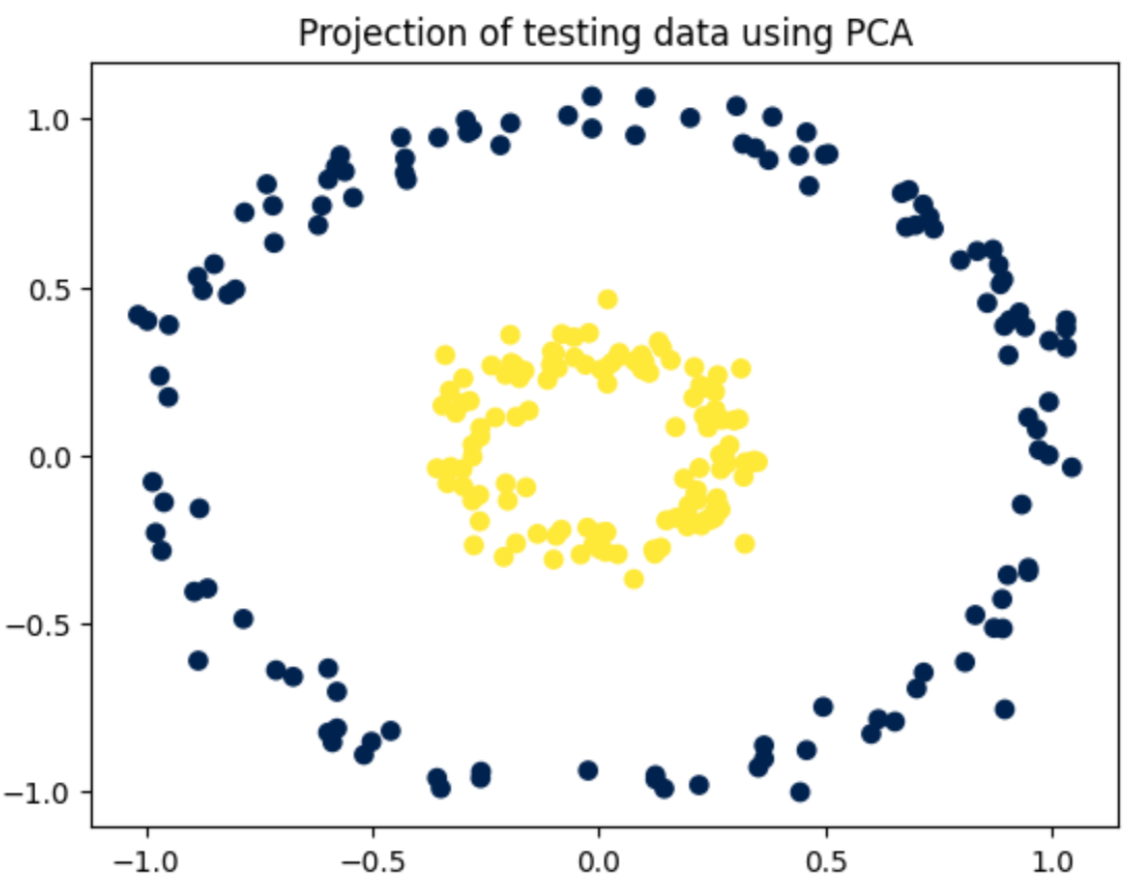
\includegraphics[width=0.5\textwidth]{figures/theory-example-figures/circles-pca.png}
    \caption{PCA on circles}
    \label{fig:circles-pca}
\end{figure}

On figure ~\ref{fig:circles-pca} it can be seen that \gls{pca}'s transformation did not manage to map the nonlinear data at all. On figure \ref{fig:circles-lda} \gls{lda} has reduced the data's dimensions to one dimension, but the two classes are clustered, which means that \gls{lda} could not separate the two classes.

\begin{figure}[htb!]
    \centering
    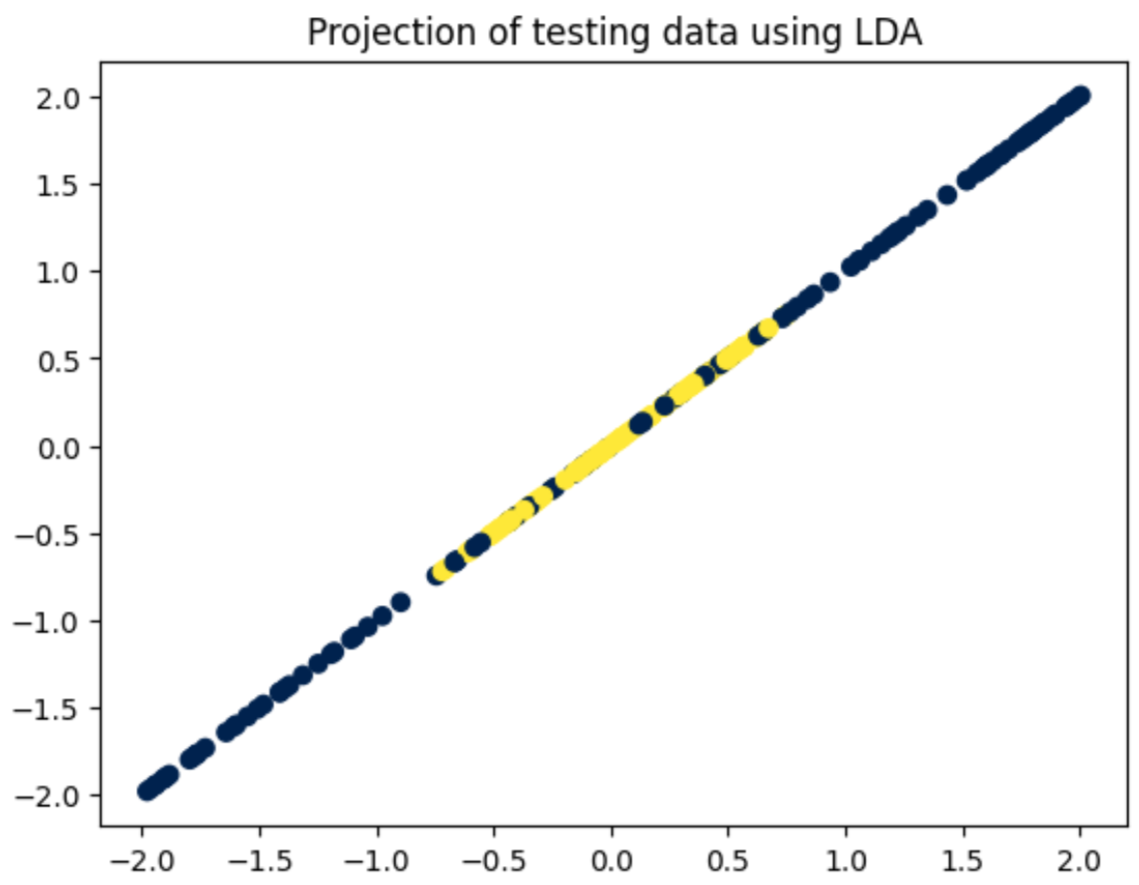
\includegraphics[width=0.5\textwidth]{figures/theory-example-figures/circles-lda.png}
    \caption{LDA on circles}
    \label{fig:circles-lda}
    \end{figure}
    
\subsubsection{Nonlinear methods}\label{subsubsec:nonlinear-methods-on-circles}
On figure \ref{fig:circles-isomap} \gls{isomap} has separated the data points from the circles. Based on the first projection Isomap is capable of separating the data, and on the second projection the method is capable of capturing more information about the outer circle, thus approximating the the original data, as the outer circle has a higher variance than the inner circle. On the second projection \gls{isomap} did not reveal that much information about the inner circle.
\begin{figure}[htb!]
    \centering
    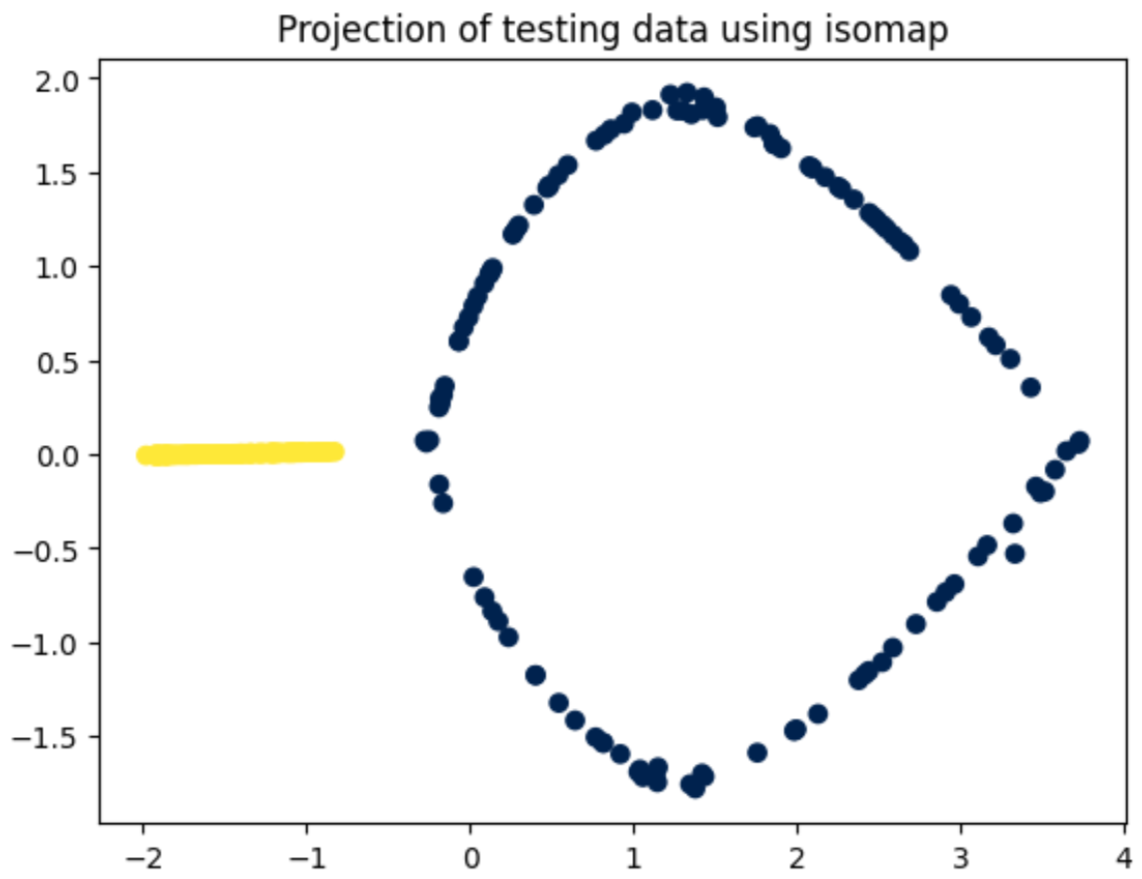
\includegraphics[width=0.5\textwidth]{figures/theory-example-figures/circles-isomap.png}
    \caption{Isomap on circles}
    \label{fig:circles-isomap}
\end{figure}


On figure \ref{fig:circles-kernelpca} \gls{kpca} has also separated the data points from the circles. \gls{kpca} does a good job at maximizing the variance for the inner circle, and also separating the the data points from each other. As it can be seen \gls{kpca} needs at least two dimensions in order to better differentiate between the two classes, as opposed to \gls{isomap}, which only needs one dimension.
\begin{figure}[htb!]
    \centering
    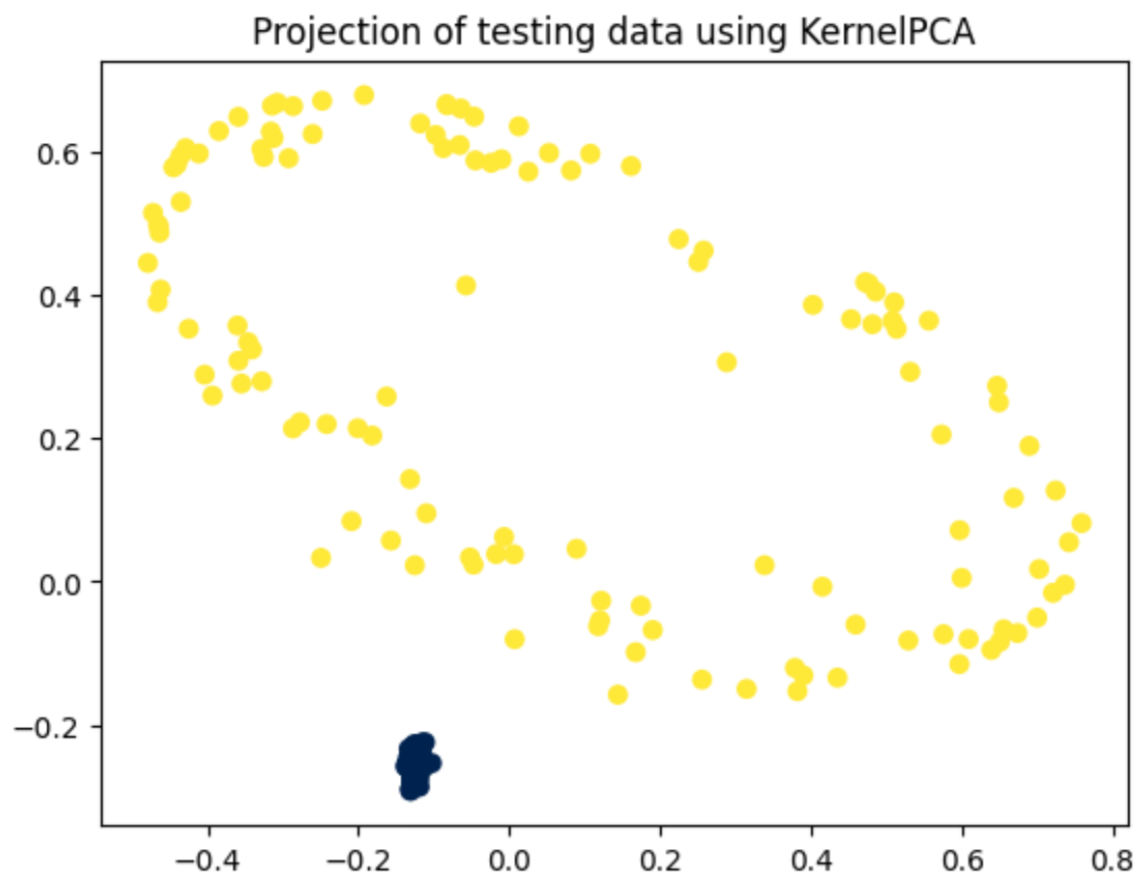
\includegraphics[width=0.5\textwidth]{figures/theory-example-figures/circles-kernelpca.png}
    \caption{KernelPCA on circles}
    \label{fig:circles-kernelpca}
\end{figure}


Until now we have presented some simple examples of the methods. More often than not, the number dimensions reduced will not be two, as there will be much more relevant information in the other dimensions too.

% @misc{iris-dataset,
% author = "Dua, Dheeru and Graff, Casey",
% year = "2017",
% title = "{UCI} Machine Learning Repository",
% url = "http://archive.ics.uci.edu/ml",
% institution = "University of California, Irvine, School of Information and Computer Sciences" }